%----------------------------------------------------------------------------------------
%    PACKAGES AND THEMES
%----------------------------------------------------------------------------------------

\documentclass[aspectratio=169,xcolor=dvipsnames]{beamer}
\usetheme{SimplePlus}

\usepackage{hyperref}
\usepackage{graphicx} % Allows including images
\usepackage{booktabs} % Allows the use of \toprule, \midrule and \bottomrule in tables
\usepackage{dsfont} % DS math font

\usepackage[T1]{fontenc}
\usepackage[polish]{babel}
\usepackage[utf8]{inputenc}



% NOTES
%-----------------------------------------------------------
\setbeameroption{hide notes} % Only slides
% \setbeameroption{show only notes} % Only notes
% \setbeameroption{show notes on second screen=right} % Both

% \setbeamertemplate{note page}{\pagecolor{yellow!5}\insertnote}\usepackage{palatino}

% CUSTOM CONSTANTS
% -----------------------------------------
\def\OT{\textlangle STA, EXP, OT\textrangle }

%----------------------------------------------------------------------------------------
%    TITLE PAGE
%----------------------------------------------------------------------------------------

\title{Learning with queries}
\subtitle{About L* algorithm}

\author{Patryk Flama}

\institute
{
    Department of Computer Science \\
    University of Wrocław
}
\date{\today}

%----------------------------------------------------------------------------------------
%    PRESENTATION SLIDES
%----------------------------------------------------------------------------------------

\begin{document}

\begin{frame}
    \titlepage
\end{frame}



\begin{frame}{Overview}
    \tableofcontents
\end{frame}


\begin{frame}[t]{Minimally Adequate Teacher}

\note{
przypomnienie co to znaczy \\
o konstrukcji takiej wyroczni; z blackboxem ciężko
}

Minimally Adequate Teacher (MAT) is an Oracle answering two types of queries:  \\

\begin{itemize}
    \item membership queries (MQ)
    \item equivalence queries (EQ)
\end{itemize}

\vspace{3mm}

$\text{QUERY} = \{\text{MQ}, \text{EQ}\}$

\end{frame}


% --------------------------------------------------------------
\section{General concept}

\begin{frame}[t]{General idea}
\begin{itemize}
    \item find a consistent observation table
    \item construct DFA and submit equivalence query to the Oracle
    \item use the counter-example to update the table
    \item submit membership queries to make the table closed and complete
    \item repeat until Oracle tells us that that the correct language has been reached
\end{itemize}

\end{frame}

% -----------------------------------------------------------
\section{Definitions}

\subsection{Observation table}
\begin{frame}[t]{Observation table}

\only<1>{

\note{
łącząc nazwę wiersza r oraz kolumny c otrzymujemy słowo rc, które należy do języka jeżeli OT[r][c] \\
jeżeli OT spełnia konkretne warunki, możemy jednoznacznie wyznaczyć dla niej DFA
}

An observation table is a specific tabular representation of an automaton

\vspace{5mm}

\begin{figure}
    \centering
    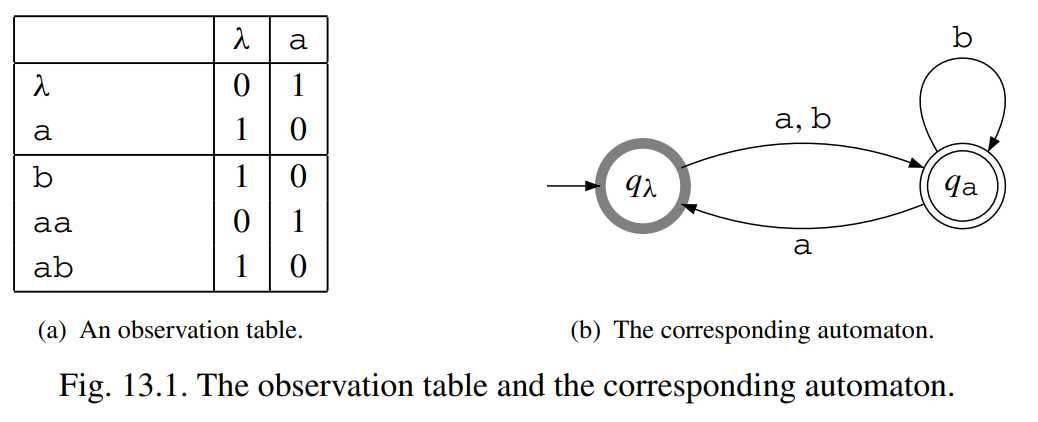
\includegraphics[width=0.75\linewidth]{images/fig13_1.png}
\end{figure}
}


\only<2>{

\note{
explain each part of OT definition (base on the book) \\
STA - zbiór słów etykietujących stany automatu \\
EXP - eksperymenty sprawdzające różnice między stanami \\
Red - tworzą podstawę automatu, każdy wiersz z Red odpowiada jednemu ze stanów w DFA \\
Blue - kandydaci na nowy stan w DFA
}

\begin{columns}
    \column{.6\textwidth}

    \begin{block}{Definition}
    An observation table is a triple \OT :
    
    \begin{itemize}
        \item $\text{STA} = \text{Red} \cup \text{Blue}$
        \item $\text{Red} \subset \Sigma^*$
        \item $\text{EXP} \subset \Sigma^*$
        \item $\text{Blue} = \text{Red} \cdot \Sigma \backslash \text{Red}$
        \item $\text{OT}: \text{STA} \times \text{EXP} \rightarrow \{0, 1, *\}$: \\
        $\text{OT}[r][c] = 
        \begin{cases}
        1 & \text{if } rc \in L \\
        2 & \text{if } rc \notin L \\
        * & \text{otherwise}
        \end{cases}$
    \end{itemize}
    \end{block}

    \column{.4\textwidth}
    \begin{figure}
        \centering
        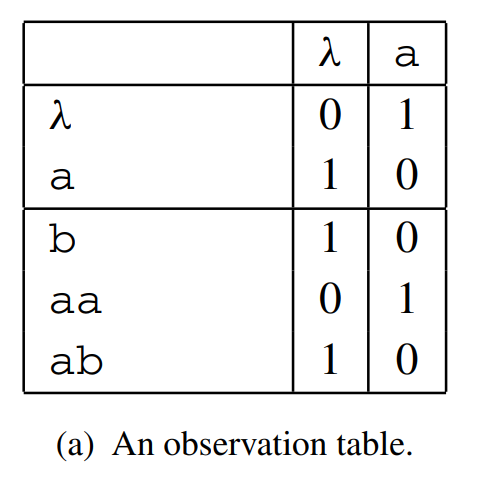
\includegraphics[width=0.9\linewidth]{images/fig13_1a.png}
    \end{figure}

\end{columns}
}

\end{frame}


\subsection{Holes and completeness}
\begin{frame}[t]{Holes and completeness}

\note{
quickly explain definitions \\
why incomplete table is a problem
}

\begin{block}{Holes}
A hole in a table \OT is a pair $(r, c)$ such that $\text{OT}[r][c] = *$
\end{block}

\begin{block}{Completeness}
A table is complete if it has no \textbf{Holes}
\end{block}

\begin{figure}
    \centering
    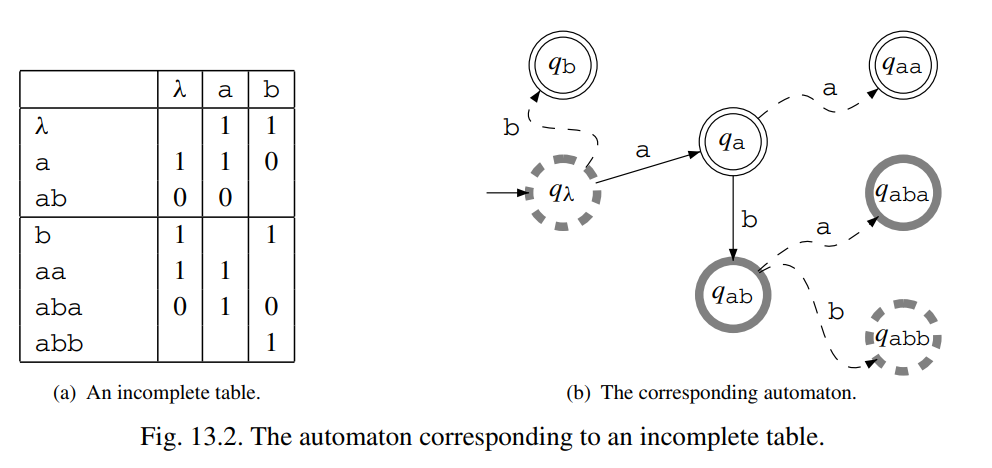
\includegraphics[width=0.6\linewidth]{images/fig13_2.png}
\end{figure}

\end{frame}



\subsection{Closed table}
\begin{frame}[t]{Closed table}

\only<1>{

\note{
równoważne <=> nie można ich odróżnić na podstawie eksperymentów z tabeli \\
tabela jest zamknięta <=> wszystkie stany z Blue są niepotrzebne (na razie) AKA póki co nie musimy ich dodawać do stanów DFA
}

We consider here the case where there are no holes in the table
\vspace{3mm}

\begin{block}{Equivalent prefixes/rows}
Two prefixes $r$ and $r'$ are equivalent if $\text{OT}[r] = OT[r']$ \\
We will denote this by $r \equiv_{\text{EXP}} r'$
\end{block}

\begin{block}{Closed table}
A table \OT is \textbf{closed} if given any row $r$ of \textit{Blue} there is some row $r'$ in \textit{Red} such that $r \equiv_{\text{EXP}} r'$
\end{block}
}

\only<2>{

\note{
intuicja: dla jakichś prefiksów i tego samego suffiksu Blue jest rozróżnialny od wszystkich z Red <=> te prefiksy muszą prowadzić do rozróżnialnego stanu \\
potem dodajemy do rozważań wszystkie nowe możliwe przejścia z tego stanu
}

It's easy to check if table is closed. But what can the algorithm do if it's not? \\
Let $r$ be the row from \textit{Blue} that does not appear in \textit{Red}. Add $r$ to \textit{Red} and $\forall a \in \Sigma$ add $ra$ to \textit{Blue} \\
We can repeat this until the table is \textbf{closed} (notice that the number of iterations is bounded by the size of the automaton)
}

\only<3>{
\begin{examples}
Row $ab$ does not appear in \textit{Red}, so we add it there. Then for all $a \in \Sigma$ ($a, b$) we add new strings to \textit{Blue}. Additionally, all known observations are filled.
\end{examples}

\begin{figure}
    \centering
    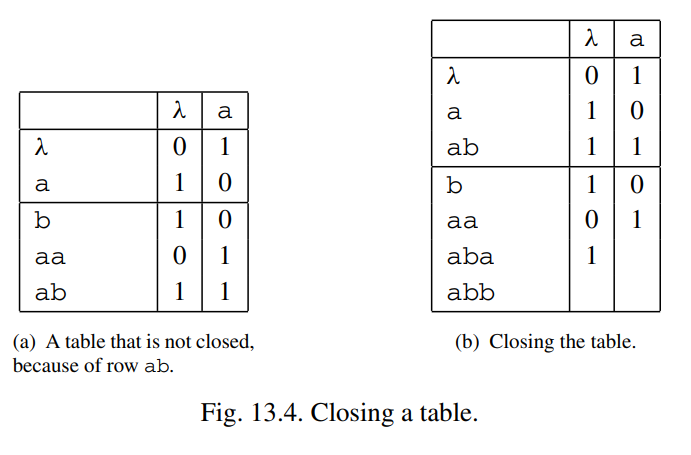
\includegraphics[width=0.6\linewidth]{images/fig13_4.png}
\end{figure}
}

\end{frame}


\section{Algorithm: build DFA from table}
\begin{frame}[t]{Build DFA from table}

\note{
prefix-closed (DEF): każdy stan automatu (który znajduje się w STA) musi mieć wszystkie swoje prefiksy w STA
}

\only<1>{
We can build DFA from observation table, if:
\begin{itemize}
    \item The set of strings marking the states in STA must be prefix-closed
    \item The set EXP is suffix-closed
    \item The table must be complete (have no holes)
    \item The table must be closed (no 'unique' blue rows)
\end{itemize}
}


\only<2>{

\note{
na razie pomiń co znaczą wymagane warunki \\
po krótce wytłumacz jak się buduje automat z OT
}

\begin{figure}
    \centering
    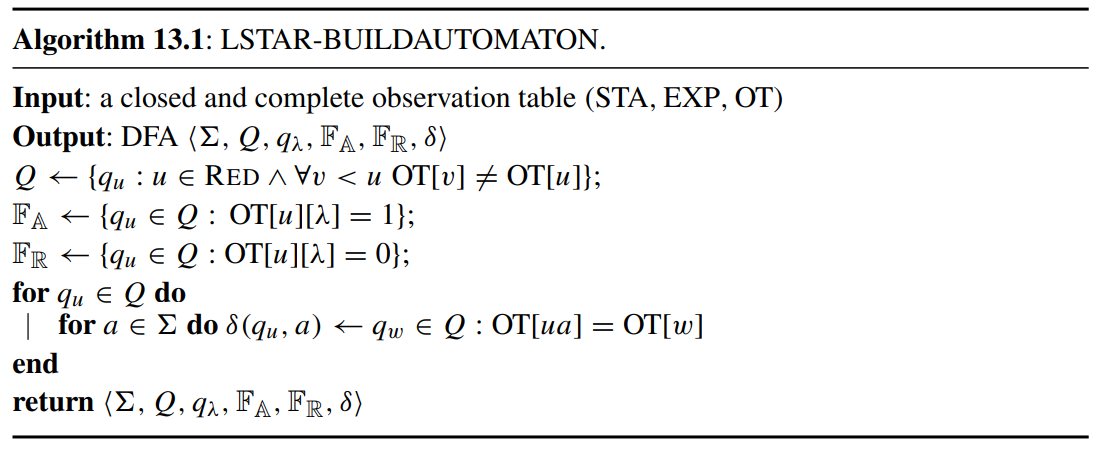
\includegraphics[width=1\linewidth]{images/alg13_1.png}
\end{figure}
}
\end{frame}

\begin{frame}[t]{Example}
After applying construction from algorithm on given table, we obtain $Q = \{q_\lambda, q_a\}, \mathds{F}_{\mathds{A}} = {q_a}, \mathds{F\mathds{R}} = {q_\lambda}$ and $\delta$ given by the transition table

\begin{columns}
    \column{.6\textwidth}
    \begin{figure}
        \centering
        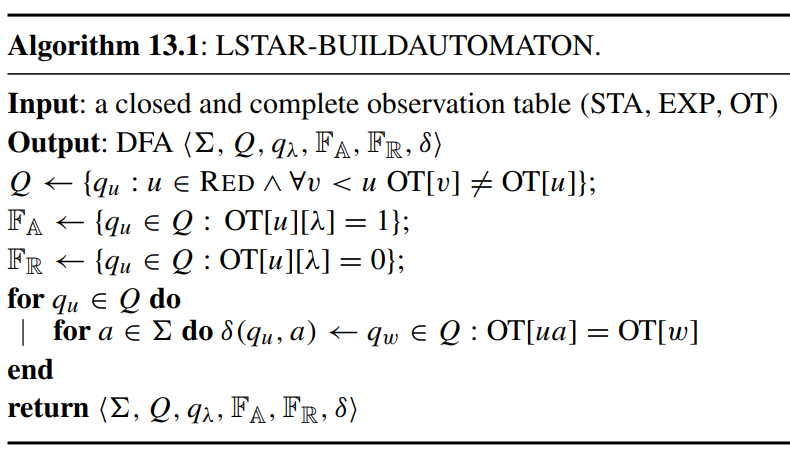
\includegraphics[width=1\linewidth]{images/alg13_1_small.png}
    \end{figure}

    \column{.2\textwidth}
    \begin{figure}
        \centering
        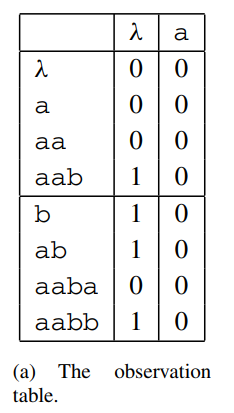
\includegraphics[width=1\linewidth]{images/fig13_3a.png}
    \end{figure}

    \column{.2\textwidth}
    \begin{figure}
        \centering
        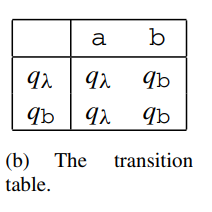
\includegraphics[width=1\linewidth]{images/fig13_3b.png}
    \end{figure}

    \begin{figure}
        \centering
        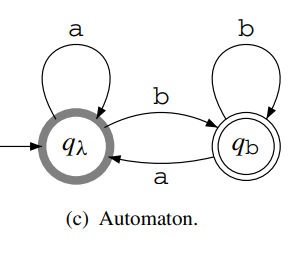
\includegraphics[width=1\linewidth]{images/fig13_3c.png}
    \end{figure}
\end{columns}

\end{frame}


\section{Consistency}
\begin{frame}[t]{Consistency}

\note{
LFA(A) is the language recognised by A by accepting states, whereas LFR(A) by rejecting states
}

\begin{block}{Consistent table (with automaton)}
Given an automaton $\mathcal{A}$ and an observation table \OT, $\mathcal{A}$ is \textbf{consistent} with table when the following holds:
\begin{itemize}
    \item $\text{OT}[r][c] = 1 \Longrightarrow rc \in \mathds{L}_{\mathds{F}_{\mathds{A}}} (\mathcal{A})$
    \item $\text{OT}[r][c] = 0 \Longrightarrow rc \in \mathds{L}_{\mathds{F}_{\mathds{R}}} (\mathcal{A})$
\end{itemize}
\end{block}

\begin{theorem}[Consistency]
Let \OT be an observation table (closed and complete). If STA is prefix-closed and EXP is suffix-closed then LSTAR-BUILDAUTOMATON(\OT) is consistent with the data in
\OT
\end{theorem}

Proof: \\
LSTAR-BUILDAUTOMATON(\OT) is built from the data from
\OT \\

\vspace{-5mm}

\rightline{$\square$}

\end{frame}


\begin{frame}[t]{Row consistency}
\only<1>{
\begin{block}{Consistent table}
A table is consistent if every equivalent pair of rows in \textit{Red} remains equivalent in STA after appending any symbol \\
$\text{OT}[r_1] = \text{OT}[r_2] \Longrightarrow \forall a \in \Sigma, \text{OT}[r_1a]= \text{OT}[r_2a]$
\end{block}

\vspace{3mm}

If table is inconsistent, then let $a \in \Sigma$ be the symbol for which the implication fails, and $e$ the experiment for which the inconsistency has been found ($\text{OT}[r_1a][e] \neq \text{OT}[r_2a][e]$) \\
Then by adding experiment $ae$ to the table, rows $r_1$ and $r_2$ are no longer equivalent ($\text{OT}[r_1][ae] \neq \text{OT}[r_2][ae]$) \\
Notice that experiments remain suffix-closed
}

\only<2>{
\begin{examples}
Table (a) is inconsistent: rows $a$ and $ab$ look the same, but, upon experiment $a$, rows $aa$ and $aba$ are different. Column  $aa$ is added, resulting in table (b) \\
Table (c) is consistent, since we have not only $\text{OT}[a] = \text{OT}[ab]$, but also $\text{OT}[aa] = \text{OT}[aba]$ and $\text{OT}[ab] = \text{OT}[abb]$
\end{examples}

\begin{figure}
    \centering
    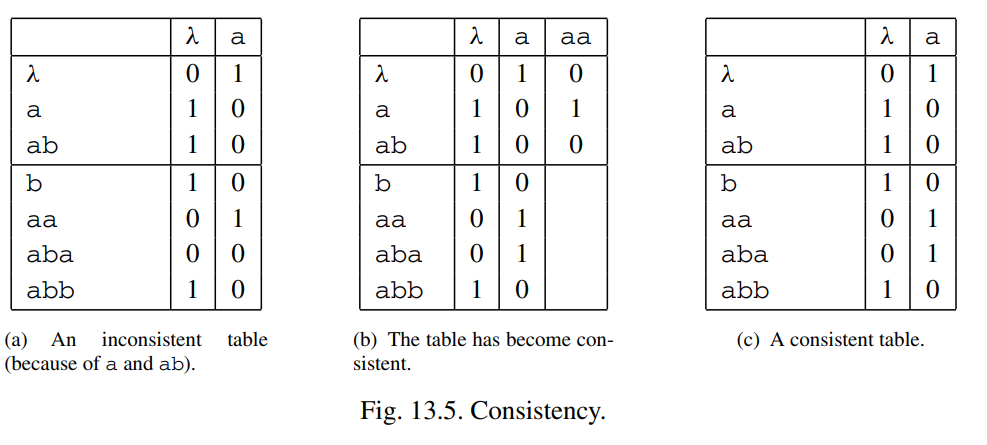
\includegraphics[width=0.7\linewidth]{images/fig13_5.png}
\end{figure}
}
\end{frame}


\begin{frame}[t]{Algorithm concept}
Once the learner has built a complete, closed and consistent table, it can construct the DFA using Algorithm LSTAR-BUILDAUTOMATON and make an equivalence query

\vspace{3mm}

If the Oracle returns a counterexample $u$, then the learner should add all prefixes of $u$ as \textit{Red} states, and complete the \textit{Blue} section, with all strings $pa$ ($a \in \Sigma$, $p$ is a prefix of $u$ but $pa$ is not) \\
In this way, at least one new \textit{Red} line has been added
\end{frame}


\section{The Algorithm}
\begin{frame}{The Algorithm}

\only<1>{

\note{
framework \\
zainicjalizuj wartości \\
spraw żeby tablica obserwacji była spójna i zamknięta \\
przetestuj rozwiązanie \\
napraw kontrprzykładem lub zwróć automat \\
}

\begin{figure}
    \centering
    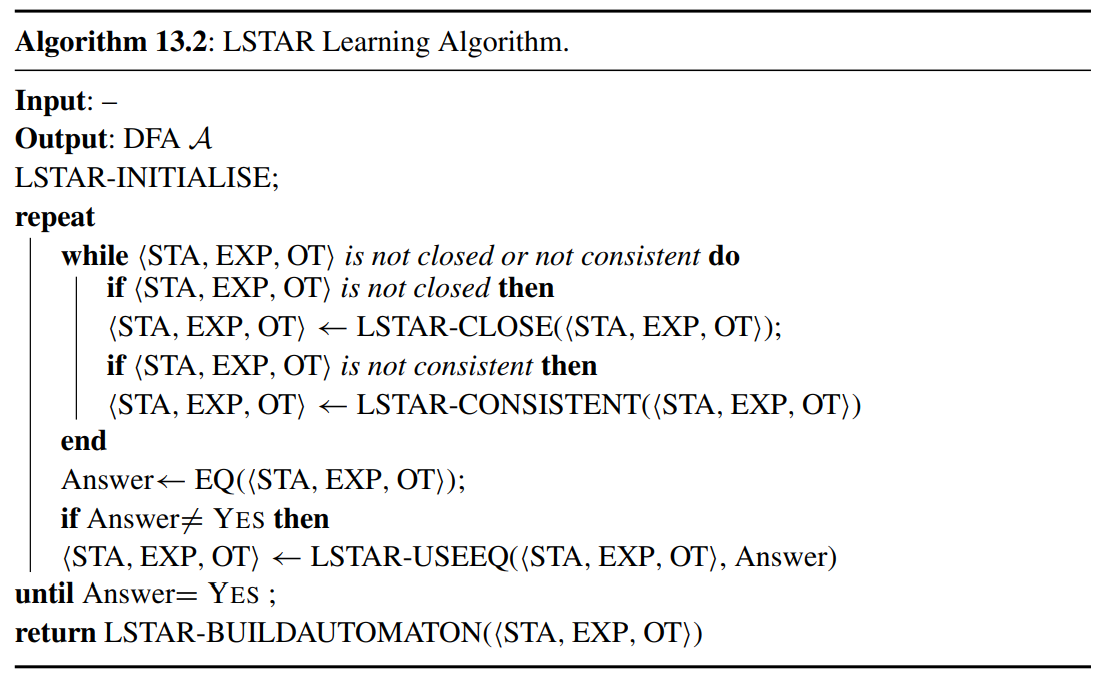
\includegraphics[width=0.8\linewidth]{images/alg13_2.png}
\end{figure}
}


\only<2>{

\note{
obserwacja: do samej budowy nie wymagamy spójności, bo nie bierzemy do niej 2 równoważnych rzędów Red
}

\begin{figure}
    \centering
    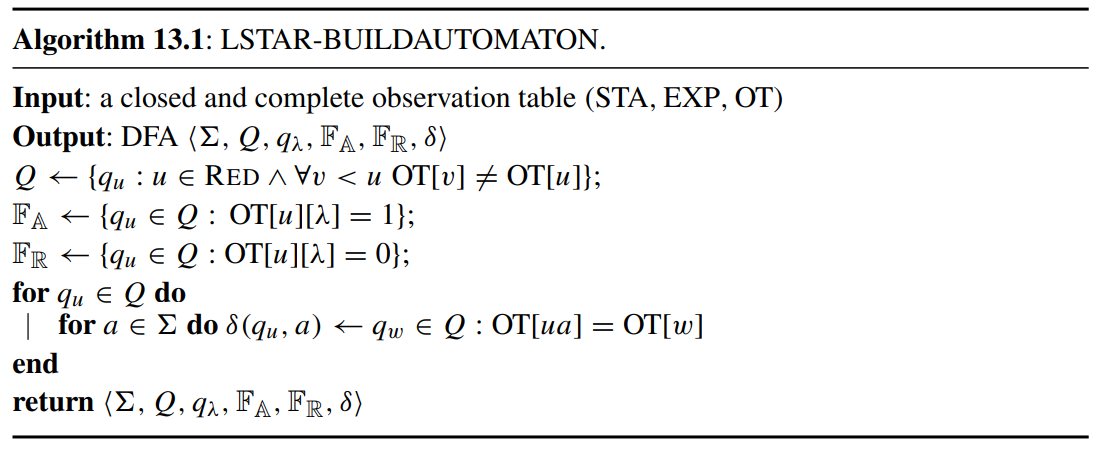
\includegraphics[width=1\linewidth]{images/alg13_1.png}
\end{figure}
}

\only<3>{

\note{
Red, EXP puste; \\
Blue wypełnione kolejnymi stanami od pustego;  \\
zawsze utrzymujemy tablicę kompletną
}

\begin{figure}
    \centering
    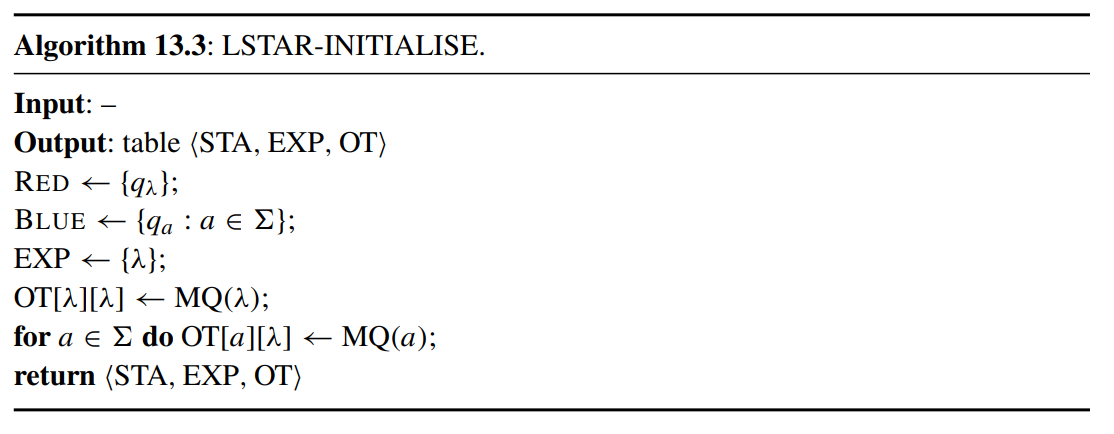
\includegraphics[width=1\linewidth]{images/alg13_3.png}
\end{figure}
}


\only<4>{

\note{
znajdź taki stan Blue że nie ma on równoważnego Red \\
przenieś go do Red, a do Blue dodaj \textit{kolejne krawędzie} \\
}

\begin{figure}
    \centering
    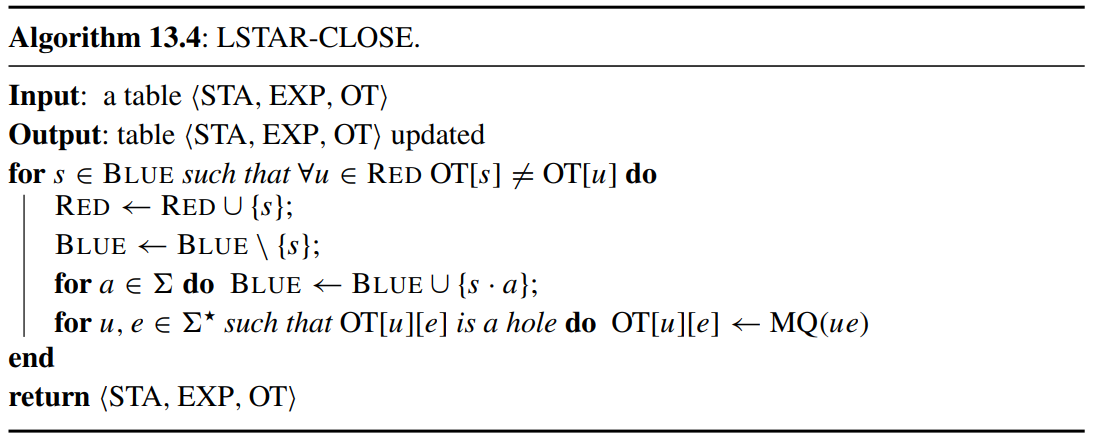
\includegraphics[width=1\linewidth]{images/alg13_4.png}
\end{figure}
}


\only<5>{

\note{
znajdź takie 2 stany Red, że są sobie równoważne, ale przejście po konkretnej \textit{krawędzi} prowadzi do niezgodności z jakimś suffiksem \\
dodaj do suffiksów tą krawędź z suffiksem (wtedy stany będą już rozróżnialne) \\
wypełnij dziury w tabeli \\
}

\begin{figure}
    \centering
    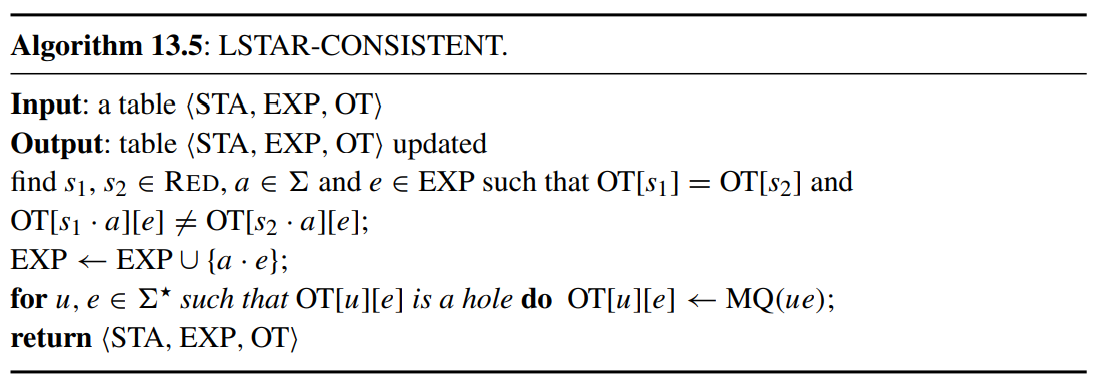
\includegraphics[width=1\linewidth]{images/alg13_5.png}
\end{figure}
}


\only<6>{

\note{
dla każdego prefiksu kontprzykładu dodaj go do Red \\
przejdź po \textit{krawędziach} i dodaj je do Blue (o ile trafią już do Red - są prefiksem kontrprzykładu)
}

\begin{figure}
    \centering
    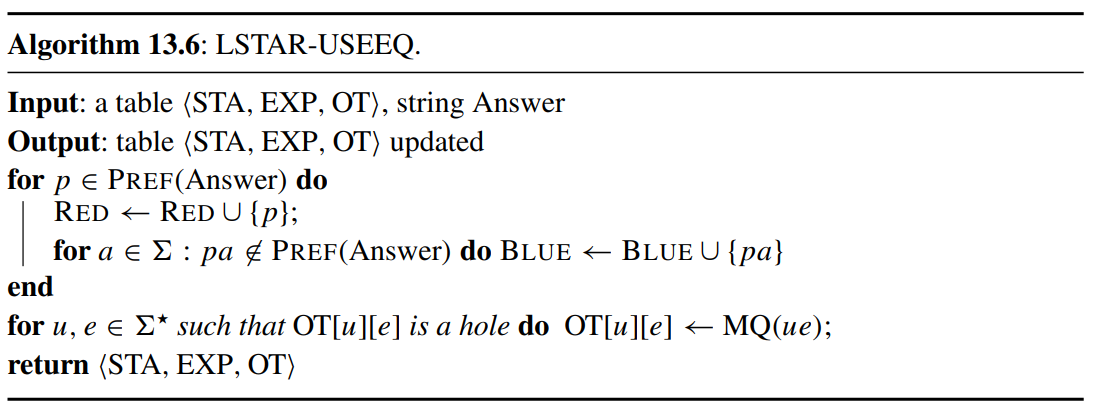
\includegraphics[width=1\linewidth]{images/alg13_6.png}
\end{figure}
}

\end{frame}


\subsection{Example}
\begin{frame}{Example}
\begin{columns}

\column{0.4\textwidth}
\begin{figure}
    \centering
    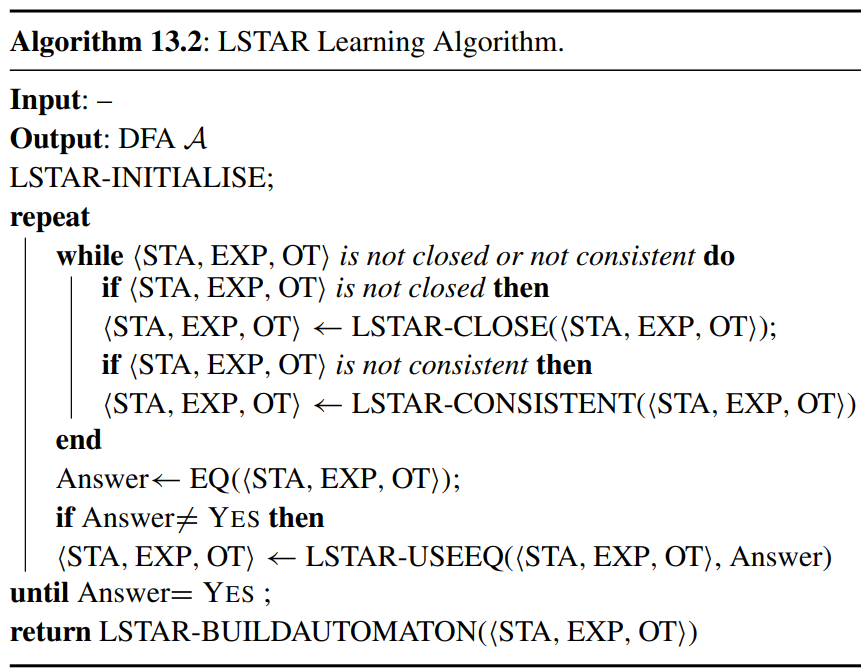
\includegraphics[width=1\linewidth]{images/alg13_2_small.png}
\end{figure}

\column{0.6\textwidth}

\only<1>{
\begin{figure}
    \centering
    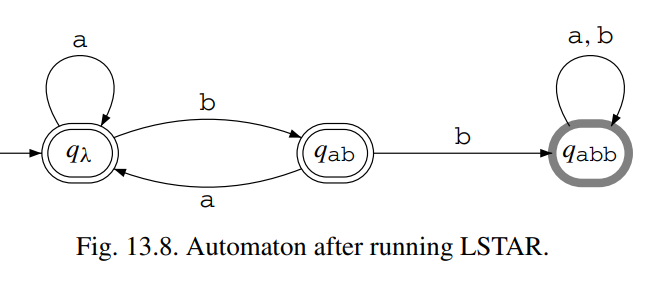
\includegraphics[width=1\linewidth]{images/fig13_8.png}
\end{figure}
}

\only<2>{

\note{
we start with empty table, and fill Blue with sigma letters - lets assume all of these are in language \\
our table is closed and complete (a) so we create automaton (b)
}

\begin{figure}
    \centering
    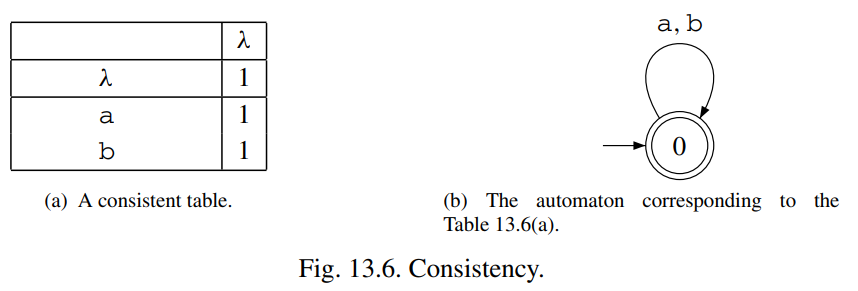
\includegraphics[width=1\linewidth]{images/fig13_6.png}
\end{figure}
}

\only<3>{

\note{
let abb be an counterexample from Oracle, we update the table (a)
we fill the holes using membership queries (b)
table (b) is not closed, because of rows a, ab and letter b; so we add expereiment b to our table; thus getting table (c)
we fill the holes (d) and get closed and cosistent table
}

\begin{figure}
    \centering
    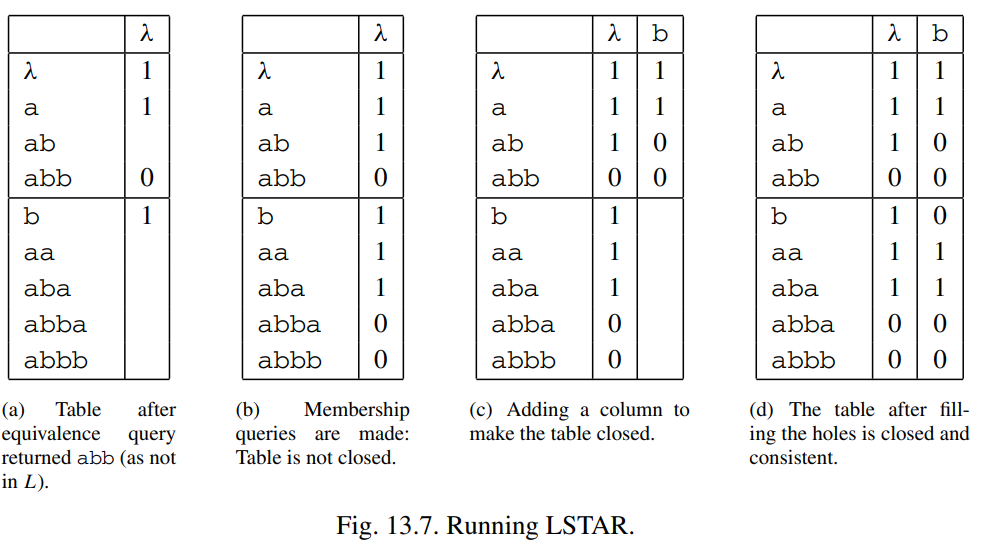
\includegraphics[width=1\linewidth]{images/fig13_7.png}
\end{figure}
}

\only<4>{

\note{
so we propose automaton from that table as solution, lets say that its accepted this time
}

\begin{figure}
    \centering
    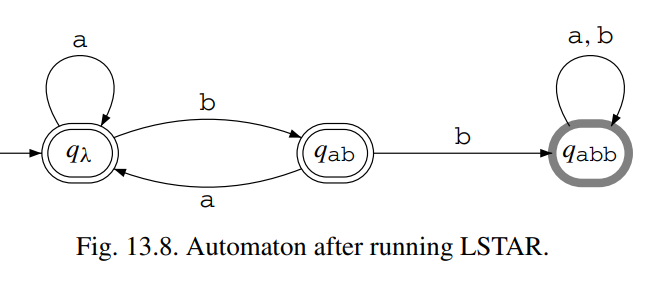
\includegraphics[width=1\linewidth]{images/fig13_8.png}
\end{figure}
}

\end{columns}
\end{frame} 


\subsection{Proof}
\begin{frame}[t]{Proof}

\note{
first we prove that with n rows we must construct a correct minimal DFA; \\
then we show that our algorithm will eventually reach n rows => it will terminate and will find the DFA \\
other words: if the algorithm has build table with n different rows in Red, and n is the size of minimal DFA for the target, then it is our target
}

We have to show that algorithm terminates, and that it returns correct automaton \\

\vspace{3mm}

Every regular language admits a unique DFA, so we can assume (wlg) that this is our target, and it has $n$ states \\
Since any DFA consistent with a table has at least as many states as different \textit{Red} rows, and construction of consistent DFA is unique, the algorithm has to end when it has $n$ rows

\begin{itemize}
    \item each closure failure adds different row to \textit{Red}
    \item each inconsistency failure adds one experiment
    \item each counterexample adds at least one different row to \textit{Red}
\end{itemize}
Thus, each time a table is inconsistent or we get a counterexample, at least one different \textit{Red} row is introduced \\
Number of steps between any of these operations i bounded, so the entire running time is bounded

\end{frame}


\subsection{Complexity}
\begin{frame}[t]{Complexity}
\begin{itemize}
    \item each experiment introduces new different \textit{Red} row, number of which is limited by $n$ $\Rightarrow |EXP| \leq n$ 
    \item for same reason at most $n$ equivalence queries are made
    \item maximal size of observation table is $n$ columns and $nm |\Sigma|$ rows ($m$ is max length of counterexample - thus it won't generate more than $nm$ \textit{Red} rows, thus there will be at most $nm |\Sigma|$ \textit{Blue} rows)
\end{itemize}

Therefore we make at most $n^2m |\Sigma|$ MQ queries and $n$ EQ queries
\end{frame}


\subsection{Implementation issues}
\begin{frame}[t]{Implementation issues}

\note{
tablica MQ posiada wyniki zapytań MQ, stały czas dostępu \\
tablica prefixów zawiera nazwy rzędów oraz ich przynależność (Red/Blue) \\
tablica eksperymentów zawiera różne eksperymenty (suffixy) \\
tablica obserwacji będzie więc symulowana funkcją OT(r, c) => MQ[rc] \\
jest to lepsze podejście bo nie trzymamy duplikatów zapytań (co mogło mieć miejsce w oryginalnej OT) \\
}

There is an issue with handling redundancy. Instead of storing an entire observation table (which could be large and inefficient), we will store 3 association tables:
\begin{itemize}
    \item MQ table
    \item Prefix (states) table
    \item Suffix (experiments) table
\end{itemize}

\vspace{3mm}

The actual observation table is simulated by a function $\text{OT}(r, c) := \text{MQ}[rc]$

\end{frame}


% \begin{frame}[t]{L\#}
% There is a relatively new algorithm L\# for learning DFA's \cite{fsharp}. \\
% It is taking a different approach, based on \textit{apartness} of states, and it is operating directly on tree-shaped automata. This simplifies the implementation and may improve learning performance (less queries to Oracle).

% \begin{columns}
%     \column{0.5\textwidth}
%     \begin{figure}
%         \centering
%         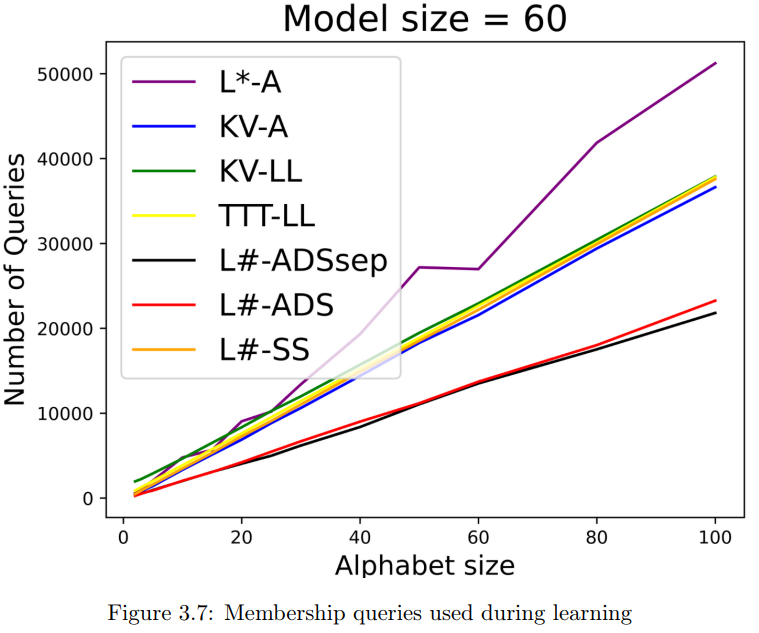
\includegraphics[width=0.8\linewidth]{images/fsharp_fig3_7.png}
%     \end{figure}

%     \column{0.5\textwidth}

%     \begin{figure}
%         \centering
%         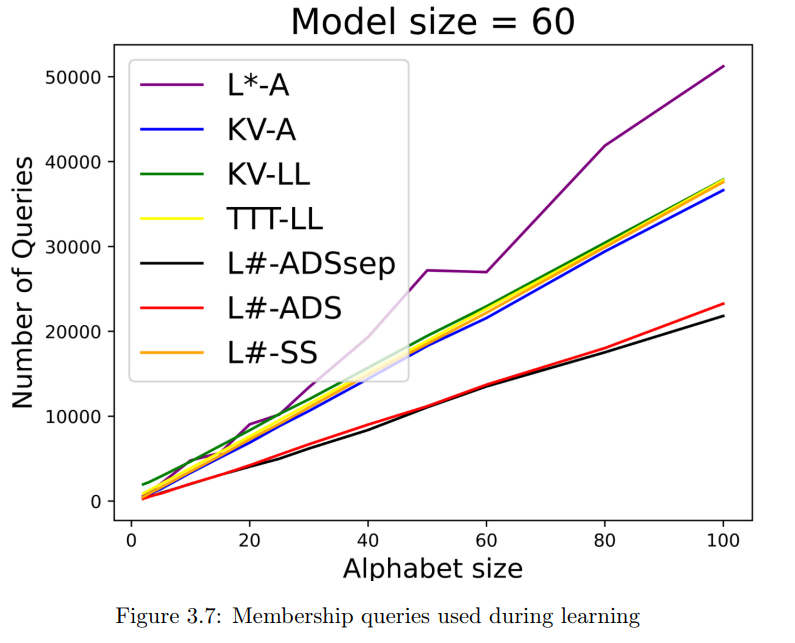
\includegraphics[width=0.8\linewidth]{images/fsharp_fig3_8.png}
%     \end{figure}
% \end{columns}

% \end{frame}


% \begin{frame}[t]{Use cases}
% % TODO: verify and gain better description/examples
% \begin{itemize}
% \item Reverse engineering
% By constructing finite automata that represent system behaviors, developers can detect discrepancies between intended and actual functionalities

% \item Network Protocol Analysis

% \item Software and Hardware verification
% \end{itemize}
% \end{frame}


\begin{frame}{Some more examples}
% TODO: jakieś zadanka

\only<1>{
\begin{figure}
    \centering
    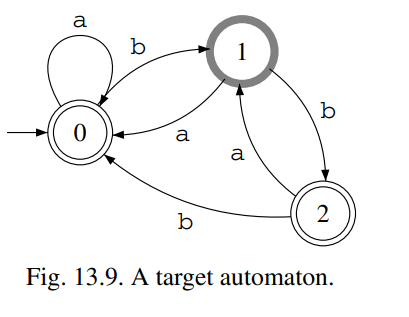
\includegraphics[width=0.5\linewidth]{images/fig13_9.png}
\end{figure}
}

\only<2>{
\begin{columns}
    \column{0.5\textwidth}
    \begin{figure}
        \centering
        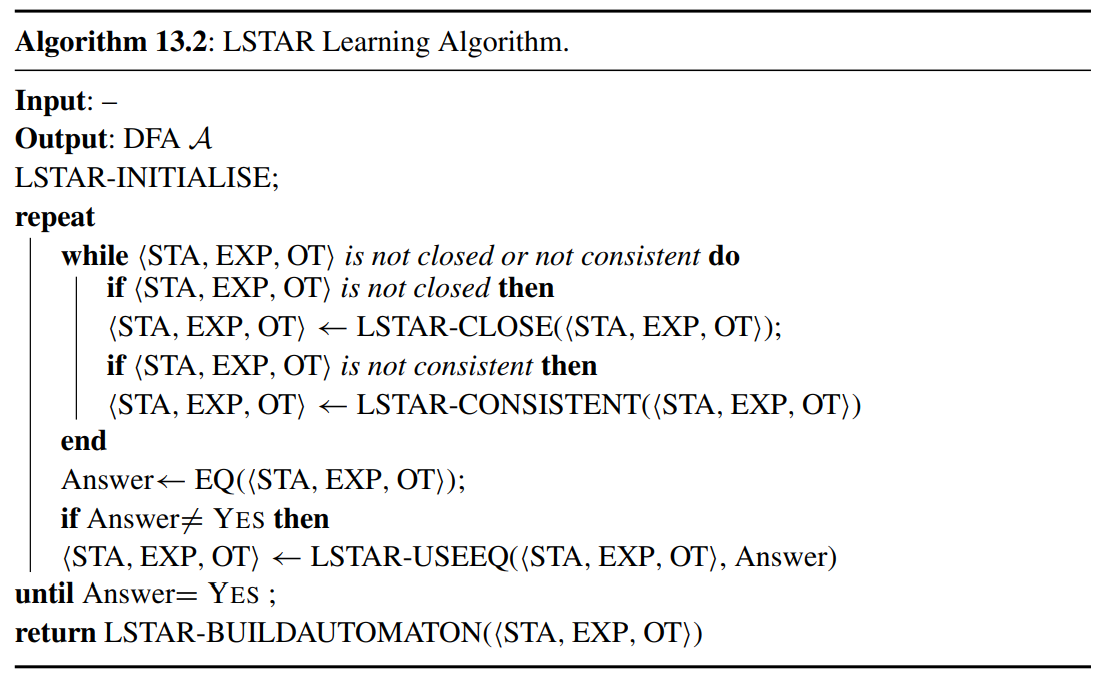
\includegraphics[width=0.9\linewidth]{images/alg13_2.png}
    \end{figure}

    \vspace{-3mm}

    \begin{figure}
        \centering
        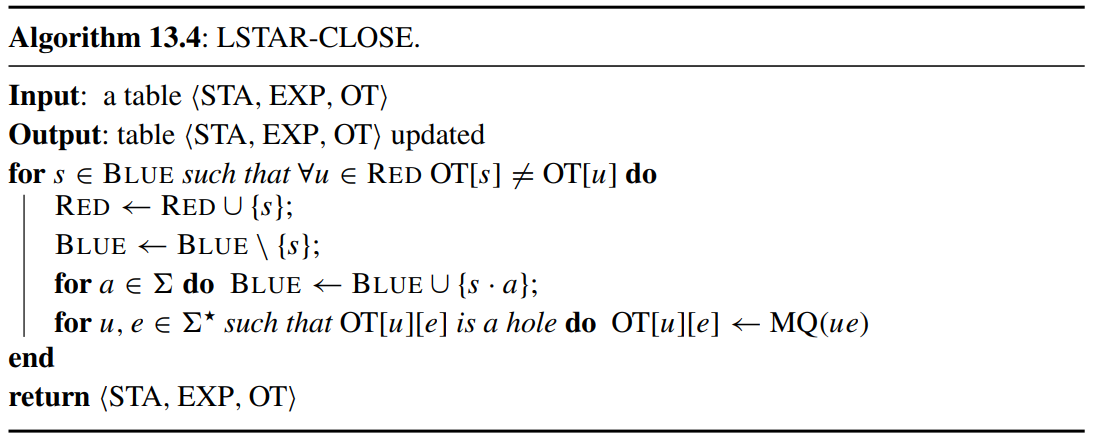
\includegraphics[width=\linewidth]{images/alg13_4.png}
    \end{figure}


    \column{0.5\textwidth}
    \begin{figure}
        \centering
        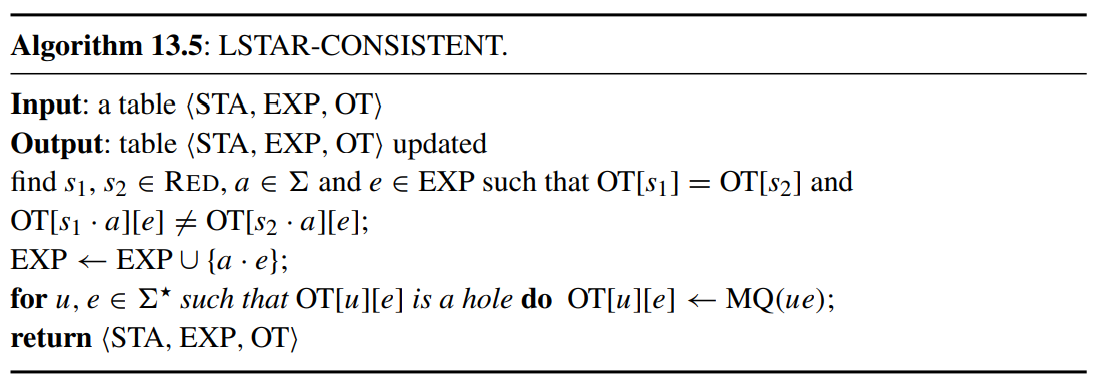
\includegraphics[width=\linewidth]{images/alg13_5.png}
    \end{figure}

    \begin{figure}
        \centering
        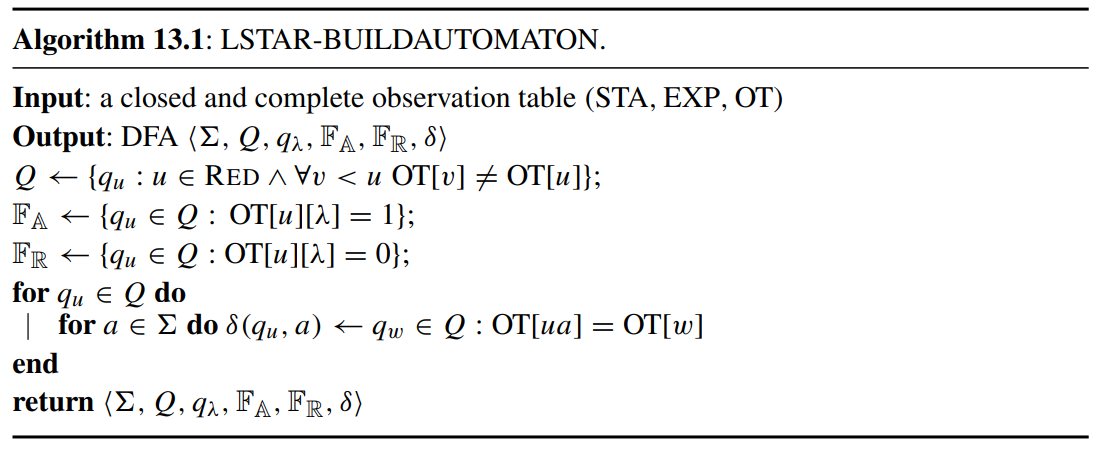
\includegraphics[width=\linewidth]{images/alg13_1.png}
    \end{figure}
\end{columns}
}
\end{frame}





% \begin{frame}{References}
%     \footnotesize
%     \bibliography{reference.bib}
%     \bibliographystyle{apalike}
% \end{frame}

\end{document}